\definecolor{bb}{RGB}{0,115,189}
\definecolor{oo}{RGB}{217,84,26}

% GNUPLOT: LaTeX picture with Postscript
\begingroup
  \makeatletter
  \providecommand\color[2][]{%
    \GenericError{(gnuplot) \space\space\space\@spaces}{%
      Package color not loaded in conjunction with
      terminal option `colourtext'%
    }{See the gnuplot documentation for explanation.%
    }{Either use 'blacktext' in gnuplot or load the package
      color.sty in LaTeX.}%
    \renewcommand\color[2][]{}%
  }%
  \providecommand\includegraphics[2][]{%
    \GenericError{(gnuplot) \space\space\space\@spaces}{%
      Package graphicx or graphics not loaded%
    }{See the gnuplot documentation for explanation.%
    }{The gnuplot epslatex terminal needs graphicx.sty or graphics.sty.}%
    \renewcommand\includegraphics[2][]{}%
  }%
  \providecommand\rotatebox[2]{#2}%
  \@ifundefined{ifGPcolor}{%
    \newif\ifGPcolor
    \GPcolorfalse
  }{}%
  \@ifundefined{ifGPblacktext}{%
    \newif\ifGPblacktext
    \GPblacktexttrue
  }{}%
  % define a \g@addto@macro without @ in the name:
  \let\gplgaddtomacro\g@addto@macro
  % define empty templates for all commands taking text:
  \gdef\gplbacktext{}%
  \gdef\gplfronttext{}%
  \makeatother
  \ifGPblacktext
    % no textcolor at all
    \def\colorrgb#1{}%
    \def\colorgray#1{}%
  \else
    % gray or color?
    \ifGPcolor
      \def\colorrgb#1{\color[rgb]{#1}}%
      \def\colorgray#1{\color[gray]{#1}}%
      \expandafter\def\csname LTw\endcsname{\color{white}}%
      \expandafter\def\csname LTb\endcsname{\color{black}}%
      \expandafter\def\csname LTa\endcsname{\color{black}}%
      \expandafter\def\csname LT0\endcsname{\color[rgb]{1,0,0}}%
      \expandafter\def\csname LT1\endcsname{\color[rgb]{0,1,0}}%
      \expandafter\def\csname LT2\endcsname{\color[rgb]{0,0,1}}%
      \expandafter\def\csname LT3\endcsname{\color[rgb]{1,0,1}}%
      \expandafter\def\csname LT4\endcsname{\color[rgb]{0,1,1}}%
      \expandafter\def\csname LT5\endcsname{\color[rgb]{1,1,0}}%
      \expandafter\def\csname LT6\endcsname{\color[rgb]{0,0,0}}%
      \expandafter\def\csname LT7\endcsname{\color[rgb]{1,0.3,0}}%
      \expandafter\def\csname LT8\endcsname{\color[rgb]{0.5,0.5,0.5}}%
    \else
      % gray
      \def\colorrgb#1{\color{black}}%
      \def\colorgray#1{\color[gray]{#1}}%
      \expandafter\def\csname LTw\endcsname{\color{white}}%
      \expandafter\def\csname LTb\endcsname{\color{black}}%
      \expandafter\def\csname LTa\endcsname{\color{black}}%
      \expandafter\def\csname LT0\endcsname{\color{black}}%
      \expandafter\def\csname LT1\endcsname{\color{black}}%
      \expandafter\def\csname LT2\endcsname{\color{black}}%
      \expandafter\def\csname LT3\endcsname{\color{black}}%
      \expandafter\def\csname LT4\endcsname{\color{black}}%
      \expandafter\def\csname LT5\endcsname{\color{black}}%
      \expandafter\def\csname LT6\endcsname{\color{black}}%
      \expandafter\def\csname LT7\endcsname{\color{black}}%
      \expandafter\def\csname LT8\endcsname{\color{black}}%
    \fi
  \fi
    \setlength{\unitlength}{0.0500bp}%
    \ifx\gptboxheight\undefined%
      \newlength{\gptboxheight}%
      \newlength{\gptboxwidth}%
      \newsavebox{\gptboxtext}%
    \fi%
    \setlength{\fboxrule}{0.5pt}%
    \setlength{\fboxsep}{1pt}%
\begin{picture}(5000.00,6000.00)%
    \gplgaddtomacro\gplbacktext{%
    }%
    \gplgaddtomacro\gplfronttext{%
      \colorrgb{0.00,0.00,0.00}%
      \put(2499,5999){\makebox(0,0){\strut{}\small Initial configuration}}%
    }%
    \gplgaddtomacro\gplbacktext{%
    }%
    \gplgaddtomacro\gplfronttext{%
      \colorrgb{0.00,0.00,0.00}%
      \put(1149,4499){\makebox(0,0){\strut{}\small FastGICP alignment progress}}%
    }%
    \gplgaddtomacro\gplbacktext{%
    }%
    \gplgaddtomacro\gplfronttext{%
      \colorrgb{0.00,0.00,0.00}%
      \put(3849,4499){\makebox(0,0){\strut{}\small FSM alignment progress}}%
    }%
    \gplgaddtomacro\gplbacktext{%
      \colorrgb{0.00,0.45,0.74}%
      \put(368,1739){\makebox(0,0)[r]{\strut{}\scriptsize $0.0$}}%
      \colorrgb{0.00,0.45,0.74}%
      \put(368,1889){\makebox(0,0)[r]{\strut{}\scriptsize $0.2$}}%
      \colorrgb{0.00,0.45,0.74}%
      \put(368,2039){\makebox(0,0)[r]{\strut{}\scriptsize $0.4$}}%
      \colorrgb{0.00,0.45,0.74}%
      \put(368,2189){\makebox(0,0)[r]{\strut{}\scriptsize $0.6$}}%
      \colorrgb{0.00,0.45,0.74}%
      \put(368,2339){\makebox(0,0)[r]{\strut{}\scriptsize $0.8$}}%
      \colorrgb{0.00,0.45,0.74}%
      \put(368,2489){\makebox(0,0)[r]{\strut{}\scriptsize $1.0$}}%
      \colorrgb{0.00,0.45,0.74}%
      \put(368,2639){\makebox(0,0)[r]{\strut{}\scriptsize $1.2$}}%
      \colorrgb{0.00,0.45,0.74}%
      \put(368,2789){\makebox(0,0)[r]{\strut{}\scriptsize $1.4$}}%

      \put(1570,2970){\makebox(0,0){\strut{}{\color{bb}{\rule[0.6mm]{0.5cm}{0.5mm}}} \footnotesize Pose estimate error}}
      \put(3370,2970){\makebox(0,0){\strut{}{\color{oo}{\rule[0.6mm]{0.5cm}{0.5mm}}} \footnotesize Internal error metric}}
    }%
    \gplgaddtomacro\gplfronttext{%
    }%
    \gplgaddtomacro\gplbacktext{%
      \colorrgb{0.15,0.15,0.15}%
      \put(857,1619){\makebox(0,0){\strut{}\scriptsize $5$}}%
      \colorrgb{0.15,0.15,0.15}%
      \put(1214,1619){\makebox(0,0){\strut{}\scriptsize $10$}}%
      \colorrgb{0.15,0.15,0.15}%
      \put(1571,1619){\makebox(0,0){\strut{}\scriptsize $15$}}%
      \colorrgb{0.15,0.15,0.15}%
      \put(1928,1619){\makebox(0,0){\strut{}\scriptsize $20$}}%
      \colorrgb{0.85,0.33,0.10}%
      \put(2131,1739){\makebox(0,0)[l]{\strut{}\scriptsize $0$}}%
      \colorrgb{0.85,0.33,0.10}%
      \put(2131,1949){\makebox(0,0)[l]{\strut{}\scriptsize $100$}}%
      \colorrgb{0.85,0.33,0.10}%
      \put(2131,2159){\makebox(0,0)[l]{\strut{}\scriptsize $200$}}%
      \colorrgb{0.85,0.33,0.10}%
      \put(2131,2369){\makebox(0,0)[l]{\strut{}\scriptsize $300$}}%
      \colorrgb{0.85,0.33,0.10}%
      \put(2131,2579){\makebox(0,0)[l]{\strut{}\scriptsize $400$}}%
      \colorrgb{0.85,0.33,0.10}%
      \put(2131,2789){\makebox(0,0)[l]{\strut{}\scriptsize $500$}}%
    }%
    \gplgaddtomacro\gplfronttext{%
    }%
    \gplgaddtomacro\gplbacktext{%
      \colorrgb{0.00,0.45,0.74}%
      \put(2868,1739){\makebox(0,0)[r]{\strut{}\scriptsize $0.0$}}%
      \colorrgb{0.00,0.45,0.74}%
      \put(2868,1889){\makebox(0,0)[r]{\strut{}\scriptsize $0.2$}}%
      \colorrgb{0.00,0.45,0.74}%
      \put(2868,2039){\makebox(0,0)[r]{\strut{}\scriptsize $0.4$}}%
      \colorrgb{0.00,0.45,0.74}%
      \put(2868,2189){\makebox(0,0)[r]{\strut{}\scriptsize $0.6$}}%
      \colorrgb{0.00,0.45,0.74}%
      \put(2868,2339){\makebox(0,0)[r]{\strut{}\scriptsize $0.8$}}%
      \colorrgb{0.00,0.45,0.74}%
      \put(2868,2489){\makebox(0,0)[r]{\strut{}\scriptsize $1.0$}}%
      \colorrgb{0.00,0.45,0.74}%
      \put(2868,2639){\makebox(0,0)[r]{\strut{}\scriptsize $1.2$}}%
      \colorrgb{0.00,0.45,0.74}%
      \put(2868,2789){\makebox(0,0)[r]{\strut{}\scriptsize $1.4$}}%
    }%
    \gplgaddtomacro\gplfronttext{%
    }%
    \gplgaddtomacro\gplbacktext{%
      \colorrgb{0.15,0.15,0.15}%
      \put(3333,1619){\makebox(0,0){\strut{}\scriptsize $2$}}%
      \colorrgb{0.15,0.15,0.15}%
      \put(3666,1619){\makebox(0,0){\strut{}\scriptsize $4$}}%
      \colorrgb{0.15,0.15,0.15}%
      \put(3999,1619){\makebox(0,0){\strut{}\scriptsize $6$}}%
      \colorrgb{0.15,0.15,0.15}%
      \put(4332,1619){\makebox(0,0){\strut{}\scriptsize $8$}}%
      \colorrgb{0.85,0.33,0.10}%
      \put(4631,1739){\makebox(0,0)[l]{\strut{}\scriptsize $0$}}%
      \colorrgb{0.85,0.33,0.10}%
      \put(4631,2002){\makebox(0,0)[l]{\strut{}\scriptsize $50$}}%
      \colorrgb{0.85,0.33,0.10}%
      \put(4631,2264){\makebox(0,0)[l]{\strut{}\scriptsize $100$}}%
      \colorrgb{0.85,0.33,0.10}%
      \put(4631,2527){\makebox(0,0)[l]{\strut{}\scriptsize $150$}}%
      \colorrgb{0.85,0.33,0.10}%
      \put(4631,2789){\makebox(0,0)[l]{\strut{}\scriptsize $200$}}%
    }%
    \gplgaddtomacro\gplfronttext{%
    }%
    \gplgaddtomacro\gplbacktext{%
    }%
    \gplgaddtomacro\gplfronttext{%
      \colorrgb{0.00,0.00,0.00}%
      \put(1149,1379){\makebox(0,0){\strut{}\small FastGICP final alignment}}%
    }%
    \gplgaddtomacro\gplbacktext{%
    }%
    \gplgaddtomacro\gplfronttext{%
      \colorrgb{0.00,0.00,0.00}%
      \put(3849,1379){\makebox(0,0){\strut{}\small FSM final alignment}}%
    }%
    \gplbacktext
    \put(0,0){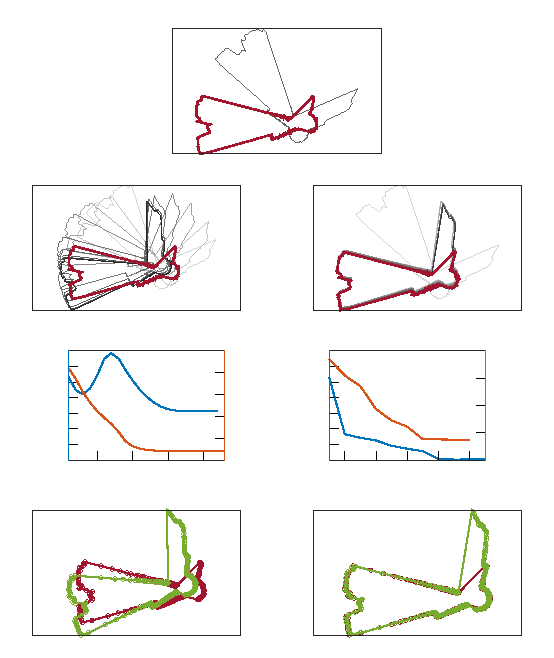
\includegraphics{./figures/characterisation/fsm_vs_fgi}}%
    \gplfronttext
  \end{picture}%
\endgroup
